% ══════════════════════════════════════════════════════════════
% CAPÍTULO 2 — MARCO CONCEPTUAL (DEFINICIÓN DE TÉRMINOS)
% Título de tesis: SISTEMA DE INTELIGENCIA ELECTORAL BASADO EN
% LLMS Y GRAFOS DE CONOCIMIENTO PARA EL ANÁLISIS MULTI-FUENTE
% DEL DISCURSO MEDIÁTICO DIGITAL: CASO ELECCIONES
% PRESIDENCIALES PERÚ 2026
% Período de datos: enero–mayo 2026
% Fuentes: YouTube (transcripciones), X/Twitter (tweets),
%           portales de noticias (scraping web), TikTok
% ══════════════════════════════════════════════════════════════

% ──────────────────────────────────────────────────────────────
\subsection{Ecosistema Digital Electoral}
% ──────────────────────────────────────────────────────────────

El ecosistema digital electoral es el conjunto de plataformas, actores y flujos de información que operan en el entorno digital durante un proceso electoral, y a través del cual los medios de comunicación, los ciudadanos y los actores políticos producen, distribuyen y consumen contenidos que construyen o transforman el discurso público sobre los candidatos \parencite{mc_chadwick2013hybrid}. A diferencia de los medios tradicionales —prensa escrita, radio y televisión—, este ecosistema se caracteriza por la descentralización de la producción de contenido, la velocidad casi instantánea de difusión y la posibilidad de interacción directa entre ciudadanos y actores políticos.

El ecosistema digital electoral está compuesto por tres tipos de actores. Los \textbf{actores institucionales} incluyen partidos políticos, candidatos y organismos electorales que utilizan las plataformas digitales de manera estratégica para comunicar sus propuestas y movilizar votantes. Los \textbf{actores mediáticos digitales} son los medios de comunicación nativos digitales, blogs especializados y portales de noticias que cubren la campaña en tiempo real, y cuya cobertura en plataformas como X/Twitter, YouTube y TikTok constituye la fuente primaria de datos de la presente investigación sobre las Elecciones Presidenciales Perú 2026. Finalmente, los \textbf{ciudadanos} generan el mayor volumen de contenido a través de sus publicaciones, comentarios y reacciones en redes sociales, constituyendo una fuente complementaria de señales del discurso político público \parencite{mc_ceron2017social}.

La comprensión de este ecosistema es fundamental para la presente investigación, ya que los datos recolectados entre enero y abril de 2026 provienen específicamente de las interacciones y publicaciones que tienen lugar en él, provenientes de cuatro fuentes: portales de noticias digitales, X/Twitter, YouTube y TikTok.

% ──────────────────────────────────────────────────────────────
\subsection{Discurso Mediático Digital}
% ──────────────────────────────────────────────────────────────

El \textbf{discurso mediático digital} es el conjunto de prácticas lingüísticas, narrativas y valorativas que los medios de comunicación producen y hacen circular a través de plataformas digitales, construyendo representaciones de la realidad política que orientan la percepción pública sobre candidatos, partidos, propuestas y el proceso electoral en su conjunto \parencite{bk_fairclough2003analysing}. A diferencia del concepto de «percepción proyectada», que pone el énfasis en la actitud evaluativa del emisor, el concepto de discurso mediático digital incorpora también las dimensiones estructurales, narrativas e ideológicas de los textos producidos: qué actores son mencionados, en qué roles, con qué relaciones entre sí, y qué marcos interpretativos se activan.

El discurso mediático digital se manifiesta de manera diferenciada según la plataforma: el lenguaje formal y estructurado de los artículos periodísticos, la brevedad y reactividad de los tweets, la oralidad transcrita de los videos de YouTube, y el registro coloquial e hipertextual de las publicaciones de TikTok configuran registros discursivos distintos que el sistema de inteligencia electoral debe ser capaz de procesar de forma integrada y comparada. El análisis multi-fuente de este discurso —habilitado por los LLMs y representado de forma estructurada en el grafo de conocimiento— es el objeto central de la presente investigación aplicada al caso de las Elecciones Presidenciales Perú 2026.

% ──────────────────────────────────────────────────────────────
\subsection{Análisis Multi-fuente}
% ──────────────────────────────────────────────────────────────

El \textbf{análisis multi-fuente} (\textit{multi-source analysis}) es el enfoque metodológico que integra y compara sistemáticamente datos provenientes de múltiples fuentes de información para obtener una comprensión más completa, robusta y triangulada de un fenómeno de interés \parencite{bk_yin2018case}. En el contexto del discurso mediático electoral, el análisis multi-fuente permite identificar qué narrativas son transversales a todo el ecosistema digital —y por tanto representan una construcción discursiva ampliamente compartida— y cuáles son exclusivas de determinadas plataformas o medios, revelando particularidades en el tratamiento informativo de cada actor.

En la presente investigación, el análisis multi-fuente se operacionaliza mediante la ingesta, normalización y análisis comparado de contenidos provenientes de cuatro fuentes digitales: portales de noticias, X/Twitter, YouTube y TikTok. La integración de estos análisis en un grafo de conocimiento compartido permite formular consultas que trascienden los silos de cada plataforma y revelan patrones discursivos sistémicos en la cobertura de las Elecciones Presidenciales Perú 2026.

% ──────────────────────────────────────────────────────────────
\subsection{Grafo de Conocimiento Electoral}
% ──────────────────────────────────────────────────────────────

Un \textbf{grafo de conocimiento electoral} es una instancia de grafo de conocimiento especializada en representar las entidades, relaciones y eventos del ecosistema político-mediático de un proceso electoral \parencite{bk_hogan2021knowledge}. En el sistema propuesto, sus nodos principales corresponden a: candidatos presidenciales, partidos políticos, propuestas programáticas, medios de comunicación, temas del discurso mediático y eventos de la campaña (debates, anuncios, escándalos). Sus aristas representan relaciones tipadas extraídas automáticamente del corpus discursivo multi-fuente por el módulo LLM, tales como: \textit{propone}, \textit{cubre\_positivamente}, \textit{cubre\_negativamente}, \textit{debatió\_sobre}, \textit{pertenece\_a}, \textit{es\_candidato\_de}.

La estructura de grafo ofrece ventajas significativas para el análisis electoral frente a la representación tabular tradicional: permite navegar eficientemente entre entidades relacionadas mediante consultas de grafo (Cypher o SPARQL), identificar comunidades de entidades fuertemente relacionadas, y detectar patrones de cobertura que solo emergen al considerar la red completa de relaciones entre medios, candidatos y temas. La Figura \ref{fig:knowledge_graph_electoral} ilustra un fragmento representativo del grafo de conocimiento electoral construido para las Elecciones Presidenciales Perú 2026.

\begin{figure}[H]
    \begin{center}
        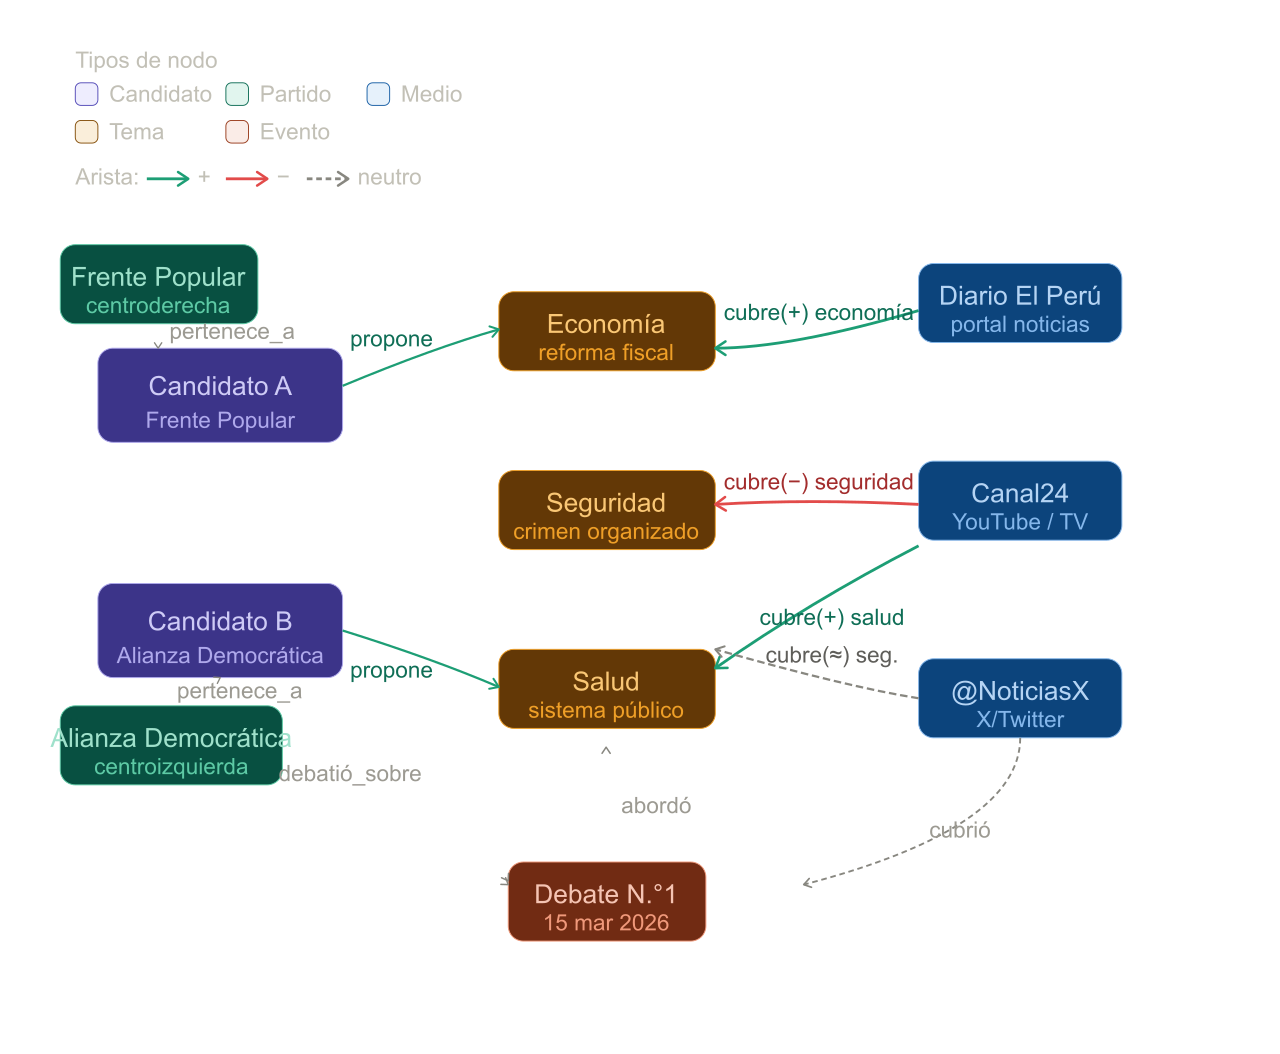
\includegraphics[width=0.88\textwidth]{2/figures/knowledge_graph_electoral.png}
        % ► NOTA PARA EL AUTOR: esta figura debe mostrar un subgrafo de ejemplo
        %   del grafo de conocimiento electoral, con nodos para candidatos,
        %   partidos, temas y medios de comunicación, y aristas tipadas que
        %   representen relaciones como "propone", "cubre_positivamente",
        %   "pertenece_a", "debatió_sobre". Ver notas_figuras.tex.
        \caption[Fragmento del grafo de conocimiento electoral — Elecciones Presidenciales Perú 2026]{Fragmento del grafo de conocimiento electoral construido para las Elecciones Presidenciales Perú 2026: nodos representando candidatos, partidos, temas y medios de comunicación, con aristas tipadas que codifican las relaciones discursivas extraídas del corpus multi-fuente por el módulo LLM.\\
            Fuente: Elaboración propia basada en \cite{bk_hogan2021knowledge}.}
        \label{fig:knowledge_graph_electoral}
    \end{center}
\end{figure}

% ──────────────────────────────────────────────────────────────
\subsection{Minería de Sentimientos}
% ──────────────────────────────────────────────────────────────

La minería de sentimientos, también conocida como análisis de sentimientos u \textit{opinion mining}, es la disciplina del Procesamiento del Lenguaje Natural orientada a identificar, extraer y cuantificar automáticamente las actitudes subjetivas expresadas en textos digitales —sean estas positivas, negativas o neutras— hacia personas, entidades, productos, eventos o temas de interés \parencite{tec_liu2012sentiment}. Va más allá de la simple clasificación de polaridad al buscar identificar también la intensidad del sentimiento, la emoción subyacente y las entidades específicas hacia las que se dirigen dichas actitudes.

En el contexto del sistema de inteligencia electoral, la minería de sentimientos permite responder preguntas como: ¿Con qué tono cubre la prensa digital a un candidato en las Elecciones Presidenciales Perú 2026? ¿Cómo varía el encuadre discursivo de los medios antes y después de un debate presidencial? ¿Qué emociones predominan en los videos de YouTube sobre una propuesta de política pública? Las respuestas a estas preguntas ofrecen información valiosa y complementaria a las encuestas convencionales para la comprensión de la dinámica del discurso mediático electoral \parencite{mc_ceron2017social}.

Formalmente, dado un conjunto de documentos $D = \{d_1, d_2, \ldots, d_n\}$, la minería de sentimientos busca asignar a cada documento $d_i$ una función de sentimiento $S(d_i, e_j) \in \{positivo, negativo, neutro\}$, donde $e_j$ representa una entidad o aspecto de interés (por ejemplo, un candidato político), como se representa en la Figura \ref{fig:sentiment_mining_process}.

\begin{figure}[H]
    \begin{center}
        \includegraphics[width=0.65\textwidth]{2/figures/sentiment_mining_process.png}
        \caption[Proceso general de la minería de sentimientos aplicada al análisis del discurso mediático electoral multi-fuente]{Proceso de minería de sentimientos en el contexto del análisis multi-fuente del discurso mediático: desde la recolección multimodal de contenidos (noticias, X/Twitter, YouTube, TikTok) hasta la generación de indicadores de sentimiento por fuente mediática y candidato, con integración al grafo de conocimiento electoral.\\
            Fuente: Elaboración propia basada en \cite{tec_liu2012sentiment}.}
        \label{fig:sentiment_mining_process}
    \end{center}
\end{figure}

% ──────────────────────────────────────────────────────────────
\subsection{Tema Relevante}
% ──────────────────────────────────────────────────────────────

En el contexto de la presente investigación, un \textbf{tema relevante} (\textit{relevant topic}) se define como un conjunto coherente de términos, conceptos y narrativas que emergen de manera recurrente en el discurso mediático digital del proceso electoral, y que refleja una preocupación, debate o acontecimiento de interés colectivo que los medios de comunicación identifican como prioritario en su agenda \parencite{mc_blei2012lda}. La relevancia de un tema se determina por su frecuencia relativa en el corpus analizado, su persistencia en el tiempo, su presencia en múltiples fuentes y plataformas, y su capacidad de articular distintas perspectivas editoriales.

Los temas relevantes en el discurso mediático de las Elecciones Presidenciales Perú 2026 pueden agruparse en varias categorías: temas programáticos (economía, salud, educación, seguridad), temas de imagen (honestidad, liderazgo, experiencia de los candidatos), temas contingentes (escándalos, revelaciones, hechos inesperados de la campaña) y temas sistémicos (confianza en las instituciones democráticas, participación ciudadana). En el grafo de conocimiento electoral, los temas relevantes se representan como nodos que se conectan con los candidatos, medios y eventos a través de aristas tipadas, permitiendo consultas estructuradas sobre qué medios abordan qué temas y con qué valoración. La capacidad de identificar y monitorear automáticamente estos temas en tiempo real —y de compararlos entre fuentes— es uno de los objetivos centrales del sistema propuesto.

% ──────────────────────────────────────────────────────────────
\subsection{Detección Dinámica de Temas}
% ──────────────────────────────────────────────────────────────

La detección dinámica de temas es la capacidad de un sistema computacional para identificar automáticamente los temas latentes presentes en un corpus de textos y rastrear su evolución a lo largo del tiempo, sin requerir etiquetado manual previo ni un conjunto predefinido de categorías temáticas \parencite{tec_grootendorst2022bertopic}. El adjetivo «dinámica» hace referencia a que el sistema es capaz de detectar no solo los temas que ya existían al inicio del período de análisis, sino también los que emergen durante el proceso como respuesta a nuevos eventos, los que se intensifican y los que decaen.

En el contexto del análisis multi-fuente del discurso mediático, la detección dinámica de temas responde a preguntas como: ¿Qué nuevos asuntos han irrumpido en la agenda de los medios esta semana? ¿Qué temas han perdido relevancia editorial? ¿Existe una correlación entre la aparición de un tema en el discurso mediático y un evento específico de la campaña presidencial? ¿Cómo difieren los temas abordados por la prensa digital respecto a los de YouTube o TikTok? Los temas detectados dinámicamente son incorporados como nodos al grafo de conocimiento electoral, enriqueciéndolo continuamente con las narrativas emergentes del discurso mediático. Este tipo de análisis es imposible de realizar manualmente a la escala del corpus recolectado entre enero y abril de 2026, de ahí la necesidad de automatizarlo mediante LLMs y modelos de topic modeling como BERTopic \parencite{tec_grootendorst2022bertopic}.

La Figura \ref{fig:dynamic_detection_concept} ilustra el concepto de detección dinámica de temas en el contexto del discurso mediático durante las Elecciones Presidenciales Perú 2026.

\begin{figure}[H]
    \begin{center}
        \includegraphics[width=0.88\textwidth]{2/figures/dynamic_detection_concept.jpg}
        \caption[Concepto de detección dinámica de temas en el discurso mediático de las Elecciones Presidenciales Perú 2026]{Representación conceptual de la detección dinámica de temas en el discurso mediático electoral: los temas emergen y decaen en función de los hitos de campaña (debates, anuncios, escándalos), siendo identificados automáticamente por el sistema a partir del corpus enero–abril 2026 e integrados al grafo de conocimiento electoral.\\
            Fuente: Elaboración propia.}
        \label{fig:dynamic_detection_concept}
    \end{center}
\end{figure}

% ──────────────────────────────────────────────────────────────
\subsection{Corpus Multimodal}
% ──────────────────────────────────────────────────────────────

En lingüística computacional y NLP, un \textbf{corpus} (plural: \textit{corpora}) es una colección estructurada y representativa de textos en formato digital, recopilados con un propósito analítico específico y que sirven como base de datos para el entrenamiento, ajuste fino o evaluación de modelos de procesamiento del lenguaje \parencite{mc_manning1999foundations}. La calidad, representatividad y tamaño del corpus son factores determinantes en la calidad de los análisis de sentimientos y detección de temas que se puedan derivar de él.

En la presente investigación se trabaja con un \textbf{corpus multimodal}, entendido como una colección que integra documentos provenientes de múltiples fuentes y formatos de comunicación. El corpus está constituido por contenidos extraídos entre enero y abril de 2026 de cuatro plataformas digitales peruanas: (1) artículos de noticias de ocho medios de comunicación, recolectados mediante scraping web; (2) publicaciones en X/Twitter de cuentas mediáticas y ciudadanas relacionadas con el proceso electoral; (3) transcripciones de videos de canales de YouTube con cobertura política; y (4) publicaciones de TikTok de cuentas de medios y creadores de contenido político. Las características de este corpus —su tamaño, composición por fuente, distribución temporal y balance temático— son descritas en detalle en el capítulo metodológico.

% ──────────────────────────────────────────────────────────────
\subsection{Token y Tokenización}
% ──────────────────────────────────────────────────────────────

Un \textbf{token} es la unidad mínima de procesamiento en la que se divide un texto para ser procesado por un modelo de NLP o un LLM. Dependiendo del tokenizador utilizado, un token puede corresponder a una palabra completa, a un subconjunto de caracteres de una palabra (\textit{subword}), a un signo de puntuación o incluso a un espacio en blanco \parencite{tec_devlin2018bert}. Los LLMs modernos utilizan tokenizadores de subpalabras como BPE (\textit{Byte Pair Encoding}) o WordPiece, que permiten manejar vocabularios abiertos y palabras fuera del vocabulario de entrenamiento.

La \textbf{tokenización} es el proceso de segmentar un texto de entrada en tokens antes de su procesamiento por el modelo, como se ilustra en la Figura \ref{fig:tokenization_example}. Este proceso es un paso previo indispensable en cualquier pipeline de NLP y tiene implicaciones directas en el rendimiento del modelo: textos en español político peruano, con sus variantes léxicas regionales y uso de jerga electoral, presentan desafíos particulares de tokenización que se ven amplificados en el corpus multimodal de esta investigación, donde coexisten el lenguaje formal de los artículos periodísticos, la informalidad de los tweets, el lenguaje oral de las transcripciones de YouTube y los neologismos frecuentes en TikTok.

\begin{figure}[H]
    \begin{center}
        \includegraphics[width=0.82\textwidth]{2/figures/tokenization_example.jpg}
        \caption[Ejemplo de tokenización de un texto político con tokenizadores de subpalabras]{Ejemplo de tokenización BPE aplicada a un texto político en español: la oración es dividida en tokens de subpalabras que el LLM puede procesar como vectores numéricos.\\
            Fuente: Elaboración propia basada en \cite{tec_devlin2018bert}.}
        \label{fig:tokenization_example}
    \end{center}
\end{figure}

% ──────────────────────────────────────────────────────────────
\subsection{Embedding o Incrustación Semántica}
% ──────────────────────────────────────────────────────────────

Un \textbf{embedding} (o incrustación semántica) es una representación vectorial densa de un token, palabra, oración o documento en un espacio de alta dimensión, donde la proximidad geométrica entre dos vectores refleja la similitud semántica entre los elementos que representan \parencite{tec_mikolov2013word2vec}. A diferencia de las representaciones dispersas como la Bolsa de Palabras o la codificación en caliente, los embeddings capturan relaciones semánticas y sintácticas complejas en un espacio de dimensión reducida.

En el contexto de la presente investigación, los embeddings cumplen dos roles fundamentales. Por un lado, los \textbf{embeddings de palabras} generados por modelos como Word2Vec o GloVe permiten calcular la similitud semántica entre términos del discurso mediático electoral y construir representaciones del vocabulario periodístico. Por otro lado, los \textbf{embeddings de oraciones} generados por modelos como Sentence-BERT \parencite{mc_reimers2019sbert} constituyen la entrada al pipeline de BERTopic para la detección dinámica de temas, capturando el significado global de cada pieza de contenido —ya sea un artículo, un tweet, un fragmento de transcripción de YouTube o un texto de TikTok— en un único vector denso. Adicionalmente, los embeddings de documentos son almacenados en pgvector para habilitar la recuperación semántica que alimenta el componente RAG del sistema, como se representa en la Figura \ref{fig:embedding_space}.

\begin{figure}[H]
    \begin{center}
        \includegraphics[width=0.80\textwidth]{2/figures/embedding_space.jpg}
        \caption[Espacio vectorial de embeddings de contenidos del discurso mediático electoral multi-fuente]{Representación del espacio vectorial de embeddings de documentos del corpus multi-fuente: contenidos semánticamente similares —independientemente de si provienen de noticias, X/Twitter, YouTube o TikTok— se agrupan en regiones próximas del espacio, facilitando la posterior detección de temas mediante clustering y la recuperación semántica para el componente RAG del sistema.\\
            Fuente: Elaboración propia basada en \cite{mc_reimers2019sbert}.}
        \label{fig:embedding_space}
    \end{center}
\end{figure}

% ──────────────────────────────────────────────────────────────
\subsection{Prompt}
% ──────────────────────────────────────────────────────────────

Un \textbf{prompt} es la instrucción textual o consulta que se proporciona como entrada a un LLM para orientar y condicionar la respuesta que este genera \parencite{tec_white2023prompt}. El diseño del prompt es el mecanismo principal a través del cual el usuario comunica al modelo la tarea que debe realizar, el contexto en el que debe operar, el formato de la respuesta esperada y las restricciones que debe respetar, todo ello sin modificar los parámetros internos del modelo.

En el contexto del sistema de inteligencia electoral, los prompts se utilizan para instrucciones como: «Analiza el encuadre discursivo de la siguiente noticia hacia el candidato X y clasifícalo como positivo, negativo o neutro, indicando los términos que sustentan tu clasificación», o «Extrae las entidades y relaciones de este fragmento discursivo para el grafo de conocimiento electoral», o «Identifica el tema principal de los siguientes fragmentos de transcripción y etiquétalo con una frase descriptiva de no más de cinco palabras». La calidad del prompt determina directamente la calidad de los resultados del sistema sobre el corpus multimodal.

Los elementos clave de un prompt bien diseñado para análisis del discurso mediático electoral incluyen: (1) la definición del \textbf{rol} del modelo («Eres un analista de medios experto en cobertura electoral latinoamericana y extracción de conocimiento estructurado»), (2) el \textbf{contexto} de la tarea (el proceso electoral analizado, el idioma, las entidades relevantes y el tipo de fuente procesada), (3) la \textbf{instrucción} específica (qué debe hacer el modelo con el texto de entrada), (4) el \textbf{formato} de la respuesta esperada (JSON estructurado con campos para fuente, candidato, sentimiento, tema, entidades para el grafo y confianza), y (5) los \textbf{ejemplos} en modalidad few-shot cuando sea necesario, como se ilustra en la Figura \ref{fig:prompt_structure}.

\begin{figure}[H]
    \begin{center}
        \includegraphics[width=0.6\textwidth]{2/figures/prompt_structure.png}
        \caption[Estructura de un prompt optimizado para análisis del discurso mediático electoral con extracción para grafo de conocimiento]{Estructura de un prompt bien diseñado para análisis del discurso mediático electoral, mostrando sus cinco componentes: rol (analista de medios y extracción de conocimiento), contexto (incluye tipo de fuente y entidades del proceso electoral peruano), instrucción, formato JSON estructurado con campos para grafo de conocimiento, y ejemplos few-shot.\\
            Fuente: Elaboración propia basada en \cite{tec_white2023prompt}.}
        \label{fig:prompt_structure}
    \end{center}
\end{figure}

% ──────────────────────────────────────────────────────────────
\subsection{Polaridad}
% ──────────────────────────────────────────────────────────────

La \textbf{polaridad} es la dimensión evaluativa fundamental del análisis de sentimientos, que indica la orientación afectiva de un texto hacia una entidad o aspecto determinado: positiva, negativa o neutral \parencite{tec_liu2012sentiment}. En el contexto del análisis multi-fuente del discurso mediático electoral, la polaridad mide si un artículo periodístico, tweet de un medio, video de YouTube o publicación de TikTok expresa apoyo, rechazo o una posición indefinida respecto a un candidato, partido político, propuesta o evento de la campaña presidencial.

Más allá de la clasificación ternaria básica (positivo / negativo / neutral), existen modelos de polaridad más granulares que incluyen escalas de intensidad —muy positivo, positivo, neutral, negativo, muy negativo— o que descomponen la polaridad en sus dimensiones emocionales constituyentes (alegría, enojo, miedo, sorpresa, tristeza, asco) siguiendo modelos como el de Plutchik \parencite{mc_plutchik1980emotion}. Los LLMs modernos son capaces de operar en este nivel de granularidad emocional, lo que constituye una ventaja significativa respecto a los clasificadores binarios clásicos.

En el presente trabajo, la polaridad se mide a nivel de aspecto (\textit{Aspect-Based Sentiment Analysis}), desagregada por entidad política y registrada como atributo de las aristas del grafo de conocimiento electoral: una misma noticia puede expresar polaridad positiva hacia la propuesta económica de un candidato y negativa hacia su gestión en seguridad, y ambas relaciones quedan codificadas como aristas tipadas y valoradas en el grafo, lo que permite consultas estructuradas sobre el balance discursivo de cada medio.

% ──────────────────────────────────────────────────────────────
\subsection{Desinformación Electoral}
% ──────────────────────────────────────────────────────────────

La \textbf{desinformación electoral} es la producción y difusión deliberada de contenido falso, engañoso o manipulado con el propósito de distorsionar la percepción pública sobre candidatos, procesos electorales o resultados, con el fin de influir en el comportamiento de los votantes o deslegitimar las instituciones democráticas \parencite{mc_wardle2017information}. Se distingue de la \textbf{desinformación involuntaria} (\textit{misinformation}), que corresponde a la difusión de contenido falso sin intención de engañar.

En el ecosistema digital, la desinformación electoral puede adoptar múltiples formas: noticias falsas fabricadas (\textit{fake news}), imágenes o videos manipulados (\textit{deepfakes}), cuentas automatizadas (\textit{bots}) que amplifican artificialmente narrativas, o titulares descontextualizados que distorsionan hechos reales \parencite{pr_chen2024combating_misinformation}. La irrupción de los LLMs ha agravado este problema al facilitar la generación masiva de texto de apariencia creíble, aunque también ha abierto nuevas posibilidades para su detección automatizada. En el corpus multi-fuente de esta investigación —que incluye videos de YouTube y contenido de TikTok— la desinformación puede presentarse además en formato audiovisual, añadiendo una capa adicional de complejidad al proceso de detección. El grafo de conocimiento electoral juega un rol central en este módulo: al contrastar el contenido analizado con los hechos y relaciones ya verificados e indexados en el grafo, el sistema puede identificar afirmaciones inconsistentes con el conocimiento estructurado acumulado.

En el sistema de inteligencia electoral propuesto, la detección de desinformación opera como un módulo complementario al análisis de sentimientos y la detección dinámica de temas, garantizando que los indicadores del discurso mediático no sean distorsionados por contenido falso amplificado artificialmente.

% ──────────────────────────────────────────────────────────────
\subsection{Framing o Encuadre Mediático}
% ──────────────────────────────────────────────────────────────

El \textbf{framing} o encuadre mediático es el proceso mediante el cual los medios de comunicación seleccionan, enfatizan y organizan ciertos aspectos de la realidad en su cobertura informativa, promoviendo interpretaciones particulares de los eventos, actores y propuestas que están cubriendo \parencite{bk_entman1993framing}. En el contexto electoral, el framing determina si una propuesta política es presentada como una solución a un problema o como una amenaza, si un candidato es descrito en términos de sus fortalezas o sus debilidades, y qué aspectos de la campaña reciben cobertura prominente.

El análisis automatizado del framing mediante LLMs y su representación en el grafo de conocimiento permite cuantificar y comparar los encuadres predominantes en distintas fuentes mediáticas, identificar consistencias y divergencias entre la prensa escrita, Twitter, YouTube y TikTok, y rastrear cómo los encuadres evolucionan a lo largo del período electoral. Este análisis constituye uno de los aportes metodológicos centrales de la presente investigación, ya que el grafo de conocimiento permite formular consultas estructuradas del tipo «¿qué medios enmarcan al candidato X principalmente en temas de seguridad con polaridad negativa?» que serían imposibles de responder con representaciones tabulares.

% ──────────────────────────────────────────────────────────────
\subsection{Polarización Política Digital}
% ──────────────────────────────────────────────────────────────

La \textbf{polarización política digital} es el fenómeno por el cual las conversaciones en ecosistemas digitales tienden a organizarse en grupos ideológicamente distantes, con escasa interacción entre ellos y con una progresiva intensificación del discurso afectivo negativo hacia el grupo contrario \parencite{mc_iyengar2019origins}. Este fenómeno, denominado también \textit{affective polarization} (polarización afectiva), es amplificado por los algoritmos de recomendación de las plataformas digitales, que tienden a reforzar las preferencias existentes de los usuarios.

En el contexto del sistema de inteligencia electoral, la medición de la polarización política digital en el discurso mediático es un indicador relevante de la calidad del ecosistema de debate público: niveles extremos de polarización en la cobertura mediática se asocian con mayor susceptibilidad a la desinformación y mayor volatilidad del comportamiento electoral \parencite{mc_iyengar2019origins}. Los LLMs permiten cuantificar la polarización a través del análisis de la distribución del sentimiento negativo entre medios con distintas líneas editoriales y del monitoreo de las narrativas contrapuestas que cada medio construye sobre los actores políticos en las cuatro plataformas analizadas. La estructura del grafo de conocimiento electoral facilita además la visualización de estas narrativas polarizadas como comunidades de nodos con orientaciones discursivas opuestas.

% ──────────────────────────────────────────────────────────────
\subsection{Monitoreo en Tiempo Real}
% ──────────────────────────────────────────────────────────────

El \textbf{monitoreo en tiempo real} (\textit{real-time monitoring}) es la capacidad de un sistema computacional para ingerir, procesar y analizar flujos continuos de datos digitales con una latencia mínima, generando resultados actualizados de manera casi instantánea \parencite{mc_stonebraker2005streaming}. En el contexto del sistema de inteligencia electoral para las Elecciones Presidenciales Perú 2026, esto significa que el sistema es capaz de detectar un cambio brusco en el tono del discurso mediático o la emergencia de un nuevo tema en el ecosistema digital en cuestión de minutos desde que el evento desencadenante ocurre, actualizando tanto los indicadores analíticos como el grafo de conocimiento electoral.

El monitoreo en tiempo real requiere una arquitectura de software que incluye: (1) un módulo de ingesta de datos en streaming (scrapers de noticias, API de X/Twitter, \textit{yt-dlp} para YouTube y TikTok), (2) un módulo de preprocesamiento y transcripción de contenido audiovisual, (3) un módulo de inferencia con el LLM que clasifica sentimientos, detecta temas y extrae entidades y relaciones para el grafo de forma paralela para cada fuente, y (4) un módulo de visualización que actualiza los dashboards en tiempo real, como se esquematiza en la Figura \ref{fig:realtime_architecture}.

\begin{figure}[H]
    \begin{center}
        \includegraphics[width=0.7\textwidth]{2/figures/realtime_architecture.png}
        \caption[Arquitectura de procesamiento multi-fuente en tiempo real para monitoreo del discurso mediático electoral]{Arquitectura del sistema de monitoreo multi-fuente del discurso mediático electoral: ingesta multimodal (noticias, X/Twitter, YouTube, TikTok), preprocesamiento y transcripción audiovisual, inferencia LLM paralela con extracción para el grafo de conocimiento, y actualización de dashboards de visualización.\\
            Fuente: Elaboración propia basada en \cite{mc_stonebraker2005streaming}.}
        \label{fig:realtime_architecture}
    \end{center}
\end{figure}

% ──────────────────────────────────────────────────────────────
\subsection{Indicadores del Discurso Mediático Electoral}
% ──────────────────────────────────────────────────────────────

Los \textbf{indicadores del discurso mediático electoral} son métricas cuantitativas derivadas del análisis del corpus digital multi-fuente que permiten operacionalizar y medir de manera sistemática las características del discurso que los medios de comunicación construyen sobre candidatos, partidos, temas y el proceso electoral en general \parencite{mc_ceron2017social}. En la presente investigación se definen los siguientes indicadores principales:

El \textbf{Índice de Sentimiento Neto} (ISN) mide la diferencia entre la proporción de documentos con sentimiento positivo y negativo hacia una entidad política en un período determinado, calculado mediante la Ecuación \ref{eq:isn}:

\begin{equation}\label{eq:isn}
\phantomsection
ISN_{(e,t)} = \frac{P_{pos}(e,t) - P_{neg}(e,t)}{P_{total}(e,t)} \times 100
\end{equation}
\myequations{Índice de Sentimiento Neto para entidades políticas}

Donde:
\begin{conditions}
P_{pos}(e,t)    & número de documentos con sentimiento positivo hacia la entidad $e$ en el período $t$ \\
P_{neg}(e,t)    & número de documentos con sentimiento negativo hacia la entidad $e$ en el período $t$ \\
P_{total}(e,t)  & número total de documentos que mencionan a la entidad $e$ en el período $t$
\end{conditions}

El ISN puede calcularse de forma global o desagregado por fuente (noticias digitales, X/Twitter, YouTube, TikTok), permitiendo comparar el tono del discurso de cada plataforma hacia cada actor político del proceso electoral peruano.

El \textbf{Índice de Relevancia Temática} (IRT) mide la importancia relativa de un tema en el corpus en un período dado, calculado como la proporción de documentos asignados a ese tema sobre el total del corpus en ese período. El \textbf{Índice de Velocidad de Emergencia} (IVE) mide la rapidez con la que un tema nuevo gana relevancia en el discurso mediático, calculado como la derivada temporal del IRT. El \textbf{Índice de Cobertura Mediática Comparada} (ICMC) mide la divergencia en el tratamiento discursivo de un mismo tema o candidato entre distintas fuentes mediáticas, permitiendo identificar sesgos de cobertura y posicionamientos editoriales diferenciados. Estos cuatro indicadores, monitoreados conjuntamente en tiempo real y representados estructuralmente en el grafo de conocimiento electoral, constituyen el núcleo analítico del sistema de inteligencia electoral propuesto para el caso de las Elecciones Presidenciales Perú 2026.